\label{chap:cannon}
\paragraph{}
The second algorithm that we implemented for matrix multiplication was Cannon's algorithm. This algorithm avoids the reduction step which is necessary in the dot\_d primitive in the case where the tiles do not encompass an entire row. This is the main advantage for Cannon's, and we believe is one of the reasons why it generally substantially outperforms the dot\_d primitive in terms of speed. Cannon's does have more stringent tiling requirements than dot\_d does, however. It requires that the matrices be tiled uniformly across a perfect square number of partitions. These two requirements mean that if a user wants to use this primitive in the middle of a long program with outputs of other operations, those outputs must either already be structured correctly, or be retiled before they can be passed as arguments to Cannon's. 
\section{Main Algorithm}
Cannon's Algorithm is structured mainly to avoid communicating partial results. It achieves this by moving the input tiles rather than the output tiles. For a computation $A=B \cdot C$, distributed on 9 localities, we have the first iteration in figure \ref{Fig_8}. 

\begin{figure}
	\centering
	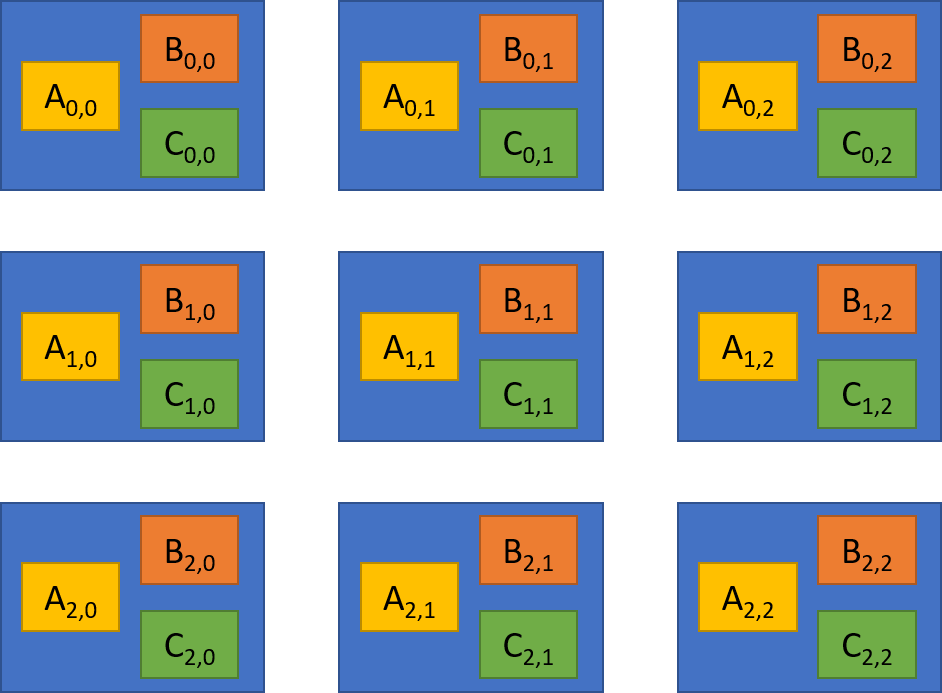
\includegraphics[width=100mm]{cannon_start}
	\caption{Starting Point of Cannon's Algorithm}
	\label{Fig_8}
\end{figure}

\begin{figure}
	\centering
	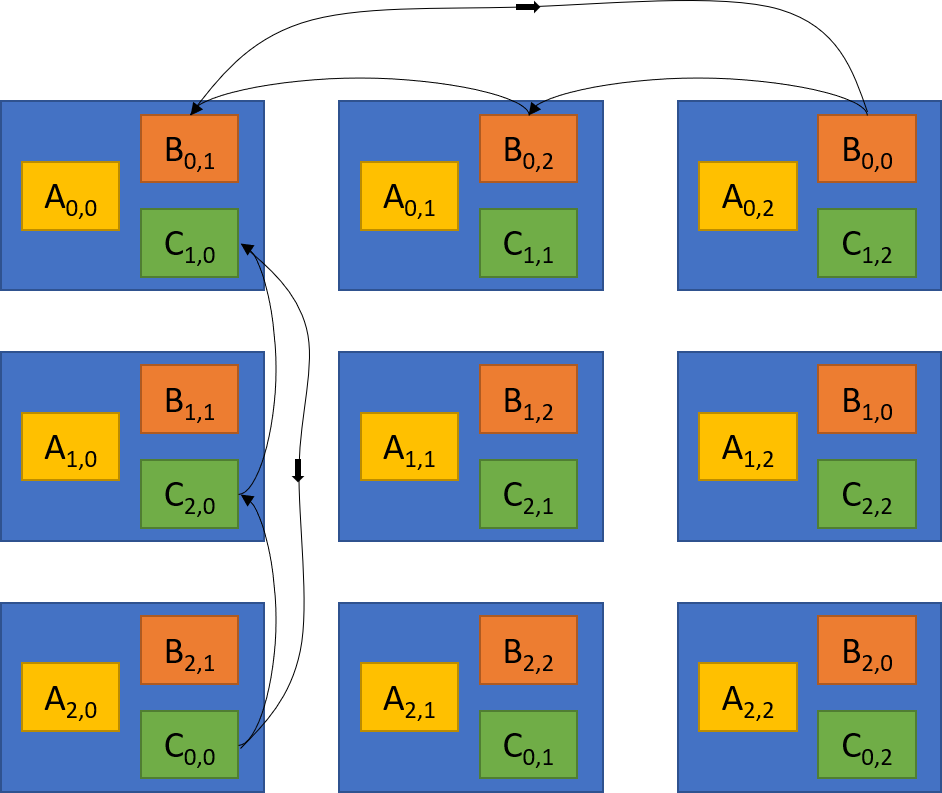
\includegraphics[width=100mm]{cannon_first_iteration}
	\caption{Data Moving}
	\label{Fig_9}
\end{figure}

Figure \ref{Fig_9} shows how after the first iteration we move the tile rows of the LHS to the left (with wraparound) and the tile columns of the RHS up (with wraparound). In the traditional formulation of Cannon's algorithm, the only loaded copy of the data is moved in each iteration. Within the design ethos of Phylanx, this would complicate the algorithm, as it introduces a hard dependency tree of move operations. For example, if node (0,0) in the tiling structure is much faster than its neighbors, it could be forced to wait until nodes (1,0) and (0,1) were done with their data so it could be moved to calculate the next partial result for (0,0). This waiting could happen at every single iteration, severely hampering execution speed. What we decided to do was not to move the sole copy of the data, but to instead use a rolling copy retrieval method, so that when the execution started, every node fetches (copies) the data to its right and below first, then the data two nodes right, and two nodes down, and so on. This does carry the cost of duplicating the tiles, but allows the the cluster to make use of all available computing capacity. 
\paragraph{}
A common practice in AMTs is to turn a single program into an execution tree composed of discrete computational units. This process allows the system to first generate the specification for all the computations needed, and perform them in order of necessity. The process of representing the computation as an execution tree is referred to as "futurizing" a computation. The term refers to the fact that intermediate results become a "future," after the standard library convention, meaning that while the result is not complete yet, you can attach computation to the result which will execute when it is complete. In order to further optimize Cannon's algorithm we chose to futurize the network communication so that we issue fetch commands on the tiles $\alpha$ we will need next, perform the multiplication on the tiles we have, issue fetch commands for the next tiles $\beta$, and perform the multiplication on the $\alpha$ tiles we fetched previously, continuing until the entire multiplication is done. 

\paragraph{}
Unlike the dot\_d primitive, the Cannon product does not have substantial difficulty in determining output tile size. Since all tiles of the LHS must be equal to each other, and since this requirement similarly holds for tiles of the RHS, the output tiles are all of the same size, that is, they will be the number of rows in a tile of $B$, by the number of columns in a tile of $C$.






%%%%%%%%%%%%%%%%%%%%%%%%%%%%%%%%%%%%%%%%%%%%%%%%%%%%%%%%%%%%%%%%%%%%%%%%%%%%%%%%%%%%%%%%%%%

%%%%%%%%%%%%%%%%%%%%%%%%%%%%%%%%%%%%%%%%%%%%%%%%%%%%%%%%%%%%%%%%%%%%%%%%%%%%%%%%%%%%%%%%%%%